\chapter{Appendices}

If there is only one appendix, it shall be labeled \textquotedblleft Appendix:\textquotedblright{}
and the appendix title. If there are more than one appendices, they
shall be labeled \textquotedblleft Appendix A: {[}title{]}\textquotedblright ,
\textquotedblleft Appendix B: {[}title{]}\textquotedblright , etc.
For software projects, appendices may include program listings, screen
shots, and sample input and output files. For hardware projects, appendices
may include printed circuit board layouts and geometric design layouts.
Other possible appendices include user manuals (created by the author
for the project), long mathematical proofs, and reviews of basic concepts.

You can insert appendices through the \textbf{Document \textgreater{}
Start Appendix Here} option. The appendix should start after the bibiliography
section of the main document. Appendices can also have chapters and
sections. \LyX{} automatically lists the appendices alphabetically.

\cleardoublepage{}

\chapter{Formatting Tips}

\section{Inserting Chapters}

On the upper left dropdown menu of the \LyX{} window, select \textit{Chapter}.
You can then type the chapter title that you want. Pressing Enter
will revert the format to \textit{Standard}, where the content can
now be placed. Chapters are numbered and placed on the \textit{Table
of Contents} automatically.

\section{Inserting Sections}

On the same dropdown menu where you insert a chapter, select \textit{Sections}.
The sections under the chapter are automatically numbered accordingly.
These also appear in the generated \textit{Table of Contents}.

\subsection{Subsections}

You can also add subsections and subsubsections. However, use them
sparingly, especially the latter.

\section{Inserting Labels}

On the chapter/section/image/table that you want to reference, click
\textbf{Insert \textgreater{} Label}. You can use the default label
that \LyX{} generates for you. To 'call' it anywhere in your document,
click the \textbf{Insert \textgreater{} Cross-reference}. This provides
an efficient way of pointing out figure/table and chapter/section
numbers, without the need to type out explicitly what the numbers
are in the document.

\section{Inserting Floats}

Figures and tables shall be included in the body of the documentation
to illustrate or clarify the accompanying text. Thus, figures and
tables must be referenced in the text in order for them to be meaningful.
By convention, figure names should be placed below the image, while
table names should be placed on top of the table. 

Moreover, figures or tables should not appear in the document before
they are mentioned in the text. By default, \LyX{} does not follow
this rule and places images or tables near, but not exactly after,
the text referencing it. You can force the rule by right-clicking
on the \textit{float:Figure} label in the \LyX{} editor and going to
\textit{Settings}. In the window that appears, shown in Figure \ref{fig:Forcing-float-placement},
uncheck \textit{Use default placement} and check \textit{Here definitely}
instead.

\begin{figure}[H]
\begin{centering}
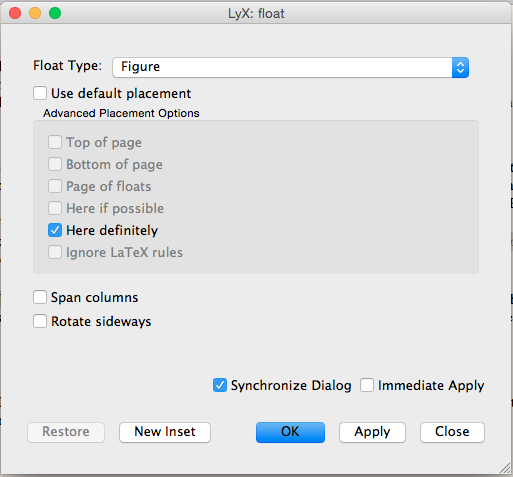
\includegraphics[width=0.5\columnwidth]{images/placement}
\par\end{centering}
\caption{Forcing float placement\label{fig:Forcing-float-placement}}

\end{figure}


\subsection{Inserting Images}

Place your cursor on the area where you want to insert the image.
Select \textbf{Insert \textgreater{} Float \textgreater{} Figure}.
Insert the actual image by selecting \textbf{Insert \textgreater{}
Graphics}. It is a recommended practice that all images should be
placed on a single folder on the same directory of this \LyX{} document
template.

You can also center the image by putting first your cursor on the
side of the image that you want to center. Right click then select
\textit{Paragraph Settings}. Finally, select the \textit{Center} button. 

You can scale the images inside the document by clicking on the image.
As shown in Figure \ref{fig:LyX-Graphics-options}, images can be
scaled relative to the column width. For two column document formats,
scale the image relative to the text width.

\begin{figure}[H]
\begin{centering}
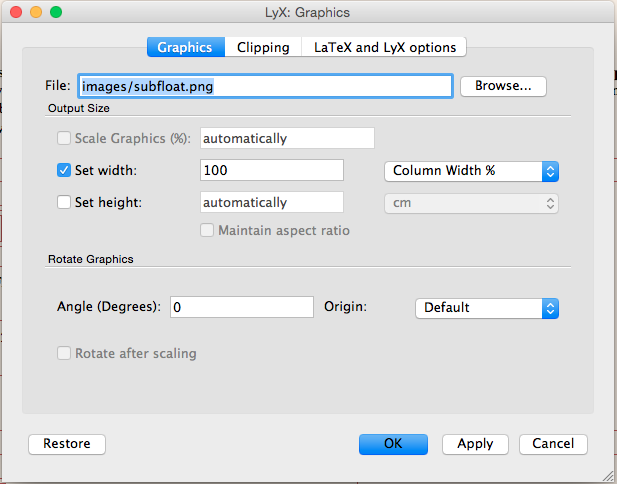
\includegraphics[width=0.6\columnwidth]{images/image_scale}
\par\end{centering}
\caption{\protect\LyX{} Graphics options\label{fig:LyX-Graphics-options}}
\end{figure}

As shown in Figure \ref{fig:Subfloat-Sample}, we can also insert
floats within the float. To put the subfloat to the document center,
click on the side of the \textit{subfloat: Figure} field, instead
of the image within the subfloat, and then access the \textit{Paragraph
Settings} as described in the previous steps. 

\begin{figure}[H]
\begin{centering}
\subfloat[Subfloat A]{\begin{centering}
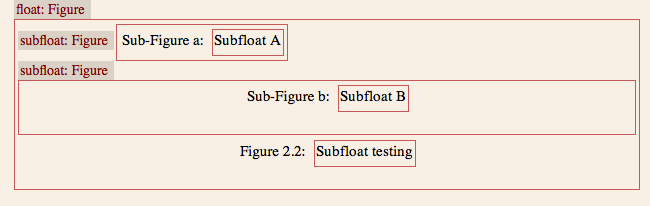
\includegraphics[width=0.8\columnwidth]{images/subfloat}
\par\end{centering}
}
\par\end{centering}
\begin{centering}
\subfloat[Subfloat B]{\begin{centering}
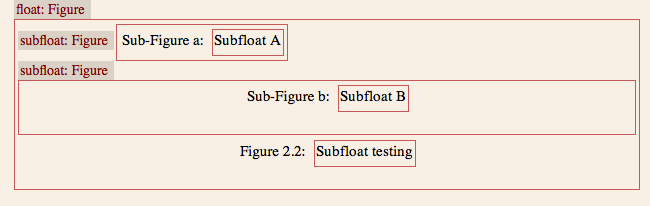
\includegraphics[width=0.8\columnwidth]{images/subfloat}
\par\end{centering}
}
\par\end{centering}
\caption{Subfloat Sample\label{fig:Subfloat-Sample}}
\end{figure}


\subsection{Inserting Tables}

Tables can be inserted just like Figure floats. Tables can also be
centered just like the images in the same way. Note that some tables
might be too long to fit the page. Again, by convention, table descriptions
are placed on top of tables as demonstrated in Table \ref{tab:Sample-Table}.
Make it fit by setting the column width (\textbf{Right click the whole
column -\textgreater{} More -\textgreater{} Settings}). 

\begin{table}[H]
\caption{Sample Table \label{tab:Sample-Table}}

\centering{}%
\begin{tabular}{|c|c|c|c|c|}
\hline 
Row 1, Column 1 & Row 1, Column 2 & Row 1, Column 3 & Row 1, Column 4 & Row 1, Column 5\tabularnewline
\hline 
\hline 
 &  &  &  & \tabularnewline
\hline 
 &  &  &  & \tabularnewline
\hline 
 &  &  &  & \tabularnewline
\hline 
 &  &  &  & \tabularnewline
\hline 
\end{tabular}
\end{table}


\section{Inserting Citations}

To download the Bib\TeX{} formatted citation from IEEEXplore, see Figure
\ref{fig:BibTeX-from-IEEEXplore}.

\begin{figure}[H]
\begin{centering}
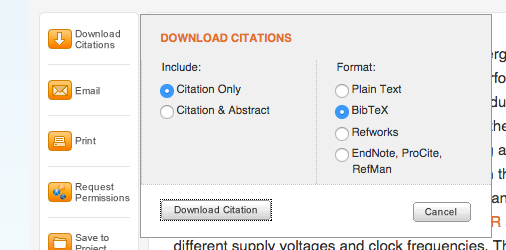
\includegraphics[width=0.55\columnwidth]{images/bibtex}
\par\end{centering}
\caption{Bib\protect\TeX{} from IEEEXplore\label{fig:BibTeX-from-IEEEXplore}}
\end{figure}

Put whatever text returned by IEEEXplore to your Bib\TeX{} file (.bib).
The references should follow the Bib\TeX{} format. To cite your paper
, click \textbf{Insert \textgreater{} Citation}, select
the desired paper, then click \textit{Add}, see Figure \ref{fig:Selecting-citations}. 

\begin{figure}[H]
\begin{centering}
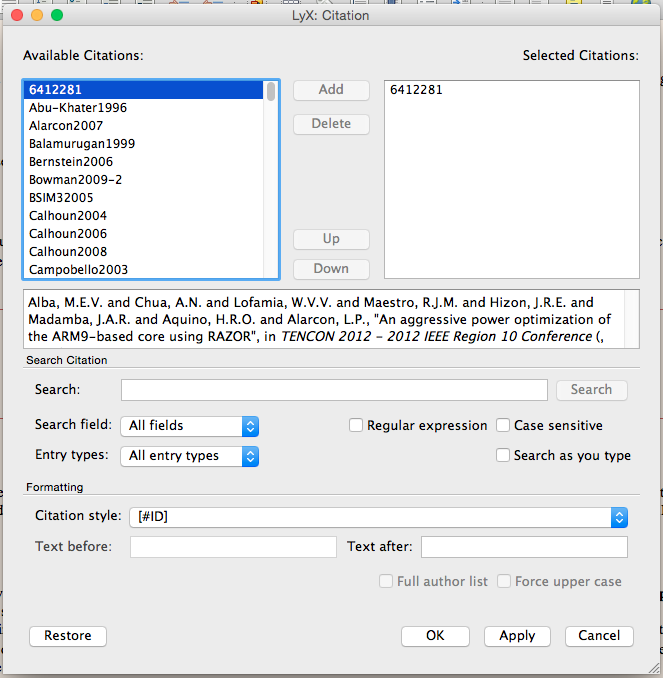
\includegraphics[width=0.7\columnwidth]{images/papers}
\par\end{centering}
\caption{Selecting citations \label{fig:Selecting-citations}}

\end{figure}

As shown in Figure \ref{fig:Bibliographies-with-no}, work titles
on bibliographies generated by Bib\TeX{} are not automatically capitalized.
Capitalization can be forced by editing the Bib\TeX{} file (.bib) and
then enclosing the capital letters of the titles with \{\}, such as
``\textbf{title=\{An \{A\}ggressive \{P\}ower \{O\}ptimization of
the \{ARM9\}-based core using \{RAZOR\}\},}''.

\begin{figure}[H]
\begin{centering}
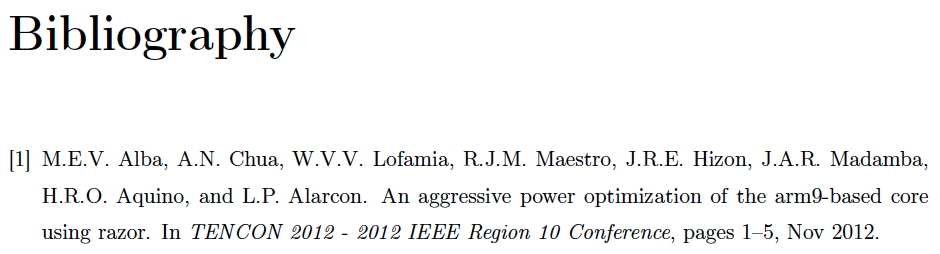
\includegraphics[width=1\columnwidth]{images/bibliography}
\par\end{centering}
\caption{Bibliographies with no auto-capitalization \label{fig:Bibliographies-with-no}}

\end{figure}

\section{Inserting Equations}

You can insert inline equations like this: $V=IR$\textbf{ }by going
to \textbf{Insert -\textgreater{} Math -\textgreater{} Inline Equation}.
You can also insert numbered equations through \textbf{Insert \textgreater{}
Math \textgreater{} Numbered Formula}. 
\begin{equation}
\nicefrac{x}{y}=\frac{x}{y}
\end{equation}

\begin{equation}
P(Z>1)=P(Z<0)=\frac{1}{2}\left[1+erf\left(\frac{Z-0.5}{\sqrt{2(0.18)}}\right)\right]=0.1193\label{eq:1}
\end{equation}

\begin{equation}
T_{P}=\frac{\left[10\unitfrac{bits}{preamble}+(4\unitfrac{bytes}{packet})(8\unitfrac{bits}{byte})\right](16\unitfrac{symbols}{bit})}{450\unitfrac{ksymbols}{second}}=1.493ms\label{eq:4-1}
\end{equation}

A math toolbar, as shown in Figure \ref{fig:Math-toolbar-for}, will
appear whenever you try to edit an equation field. This greatly helps
in creating professional-looking equations. It is required that all
equations appearing in the document be written out using this option.

\begin{figure}[H]
\begin{centering}
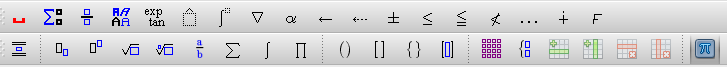
\includegraphics[width=0.9\columnwidth]{images/equations}
\par\end{centering}
\caption{Math toolbar for equation writing\label{fig:Math-toolbar-for}}

\end{figure}